\documentclass[tikz,border=10pt]{standalone}
\usepackage[scaled=0.95]{helvet}
\renewcommand{\familydefault}{\sfdefault}
\usepackage[europeanresistors,americanvoltages]{circuitikz}
\usetikzlibrary{arrows.meta,positioning}
\definecolor{TEJNavy}{HTML}{1E2B55}
\definecolor{TEJBlue}{HTML}{1769AA}
\definecolor{TEJRed}{HTML}{A43737}
\definecolor{TEJLight}{HTML}{EEF6F8}
\begin{document}
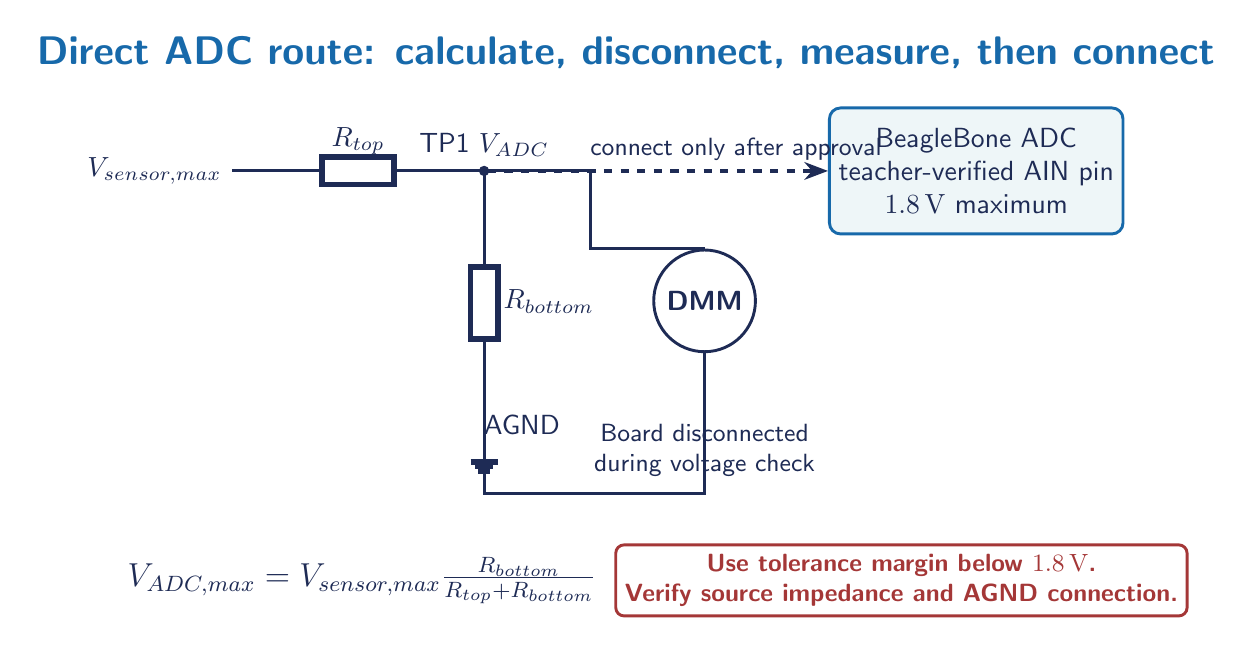
\begin{tikzpicture}[line width=1.05pt,draw=TEJNavy,text=TEJNavy,font=\sffamily]
  \ctikzset{bipoles/length=1.15cm}
  \node[font=\bfseries\Large,text=TEJBlue] at (6.0,6.85)
    {Direct ADC route: calculate, disconnect, measure, then connect};

  \draw (1.0,5.35) node[left,font=\bfseries] {$V_{sensor,max}$}
    to[R,l={$R_{top}$}] (4.2,5.35)
    node[circ,label=above:{TP1 $V_{ADC}$}] (tp) {}
    to[R,l={$R_{bottom}$}] (4.2,2.0)
    node[ground] {AGND};

  \node[draw=TEJNavy,circle,minimum size=1.25cm,font=\bfseries] (dmm) at (7.0,3.7) {DMM};
  \draw (tp) -- (5.55,5.35) |- (dmm.north);
  \draw (dmm.south) |- (4.2,1.25) -- (4.2,2.0);
  \node[align=center,font=\small] at (7.0,1.8) {Board disconnected\\during voltage check};

  \node[draw=TEJBlue,rounded corners=4pt,fill=TEJLight,minimum width=2.9cm,minimum height=1.6cm,align=center]
    (adc) at (10.45,5.35) {BeagleBone ADC\\teacher-verified AIN pin\\$1.8\,\mathrm{V}$ maximum};
  \draw[-{Stealth[length=3mm]},line width=1.25pt,dashed] (tp) -- (adc.west);
  \node[above,font=\small] at (7.4,5.35) {connect only after approval};

  \node[font=\large] at (2.65,0.15)
    {$V_{ADC,max}=V_{sensor,max}\frac{R_{bottom}}{R_{top}+R_{bottom}}$};
  \node[draw=TEJRed,text=TEJRed,rounded corners=3pt,align=center,font=\bfseries\small]
    at (9.5,0.15) {Use tolerance margin below $1.8\,\mathrm{V}$.\\Verify source impedance and AGND connection.};
\end{tikzpicture}
\end{document}
